% $Id: installation.tex,v 1.19 2008-02-26 17:07:03 mgmarino Exp $
% created by Mike
% added installation guide for CLHEP, Geant4, ROOT and MGDO by Jing
% 2007.09.10 Jing. added guide on how to get MaGe and MGDO from CVS.
% 2007.10.30 Jing. added guide on how to compile MaGe with GDML.
% 2010.10.01 Alex. update on configuration concerning newest geant4 and SVN

\section{Dependencies}
\mage depends upon the following software packages:
\begin{enumerate}
\item {} GEANT4. An installation of CLHEP is required for
  GEANT4. \mage works for CLHEP 1.9.x.x and later.
\item {} ROOT.
\item {} MGDO. MGDO stands for Majorana Gerda Data
  Objects. It defines the common data structure shared by MaGe and the
  PSS (pulse shape simulation) and PSA (pulse shape analysis)
  packages.
\item {} Optional accessories: PostgreSQL, GDML, etc.
\end{enumerate}
Fig. \ref{fig:dep} shows the dependencies graphically.

\begin{figure}[htbp]
  \centering
  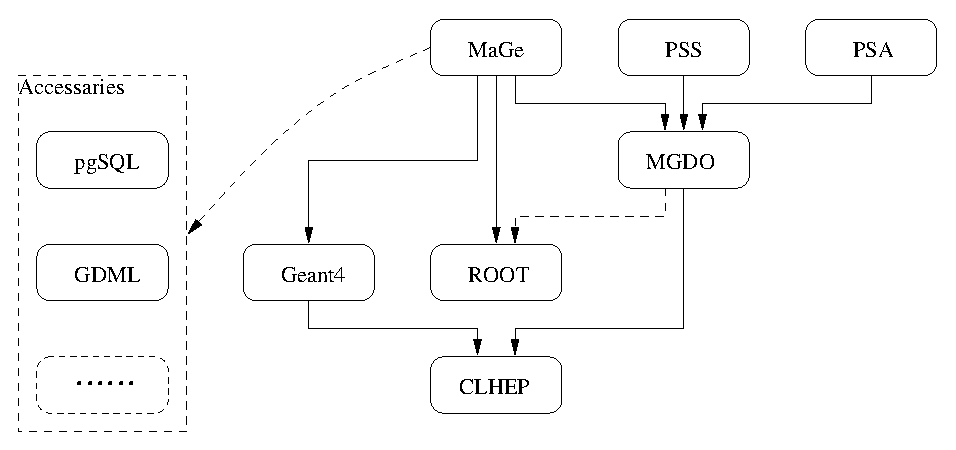
\includegraphics[width=.5\textwidth]{dependency}
  \caption{The dependencies of the software packages. Dotted lines
    indicate the optional dependencies.}
  \label{fig:dep}
\end{figure}

The dependencies determine the order of the installation, that is,
\begin{enumerate}
\item CLHEP
\item GEANT4
\item ROOT
\item MGDO
\item \mage
\end{enumerate}

\section{Getting the Packages}

\subsection{Getting CLHEP}
The \textbf{C}lass \textbf{L}ibrary for \textbf{H}igh \textbf{E}nergy \textbf{P}hysics is required for running \geant.
Go to the CLHEP web site to obtain the installation package (there are precompiled versions available):
\begin{lstlisting}
http://proj-clhep.web.cern.ch/proj-clhep/DISTRIBUTION
\end{lstlisting}
download a version newer than 1.9.x.x (2.0.4.5 is recommended by Geant4.9.3p02).

\subsection{Getting \geant}
Go to the GEANT4 web site:
\begin{lstlisting}
http://geant4.web.cern.ch/geant4/
\end{lstlisting}
download the newest version of GEANT4. If there are patches for this version,
please download them as well. GEANT4 is under development all the
time. The newer the version is, the less bugs there are.
Move the tar balls of the source codes and the patches (if there are
some) to the directory where you want to install GEANT4. Unpack the
source codes (taking version 4.8.2 as an example):
\begin{lstlisting}
  tar xfvz geant4.8.2.gtar.gz
\end{lstlisting}
Unpack the patch in the same directory:
\begin{lstlisting}
  tar xfvz patch_geant4.8.2.p01.gtar.gz
\end{lstlisting}
which will add or modify some of the GEANT4 source files.

Download the newest data files on the same web page where you download
GEANT4 source codes. Unpack them into a certain directory. Later in
the GEANT4 installation process you will be asked the place where you
put these data files.

\subsection{Getting ROOT}
To install ROOT from source you first have to get the tar file containing the source. This tar file can be found at:
\begin{lstlisting}
http://root.cern.ch/twiki/bin/view/ROOT/Download
\end{lstlisting}
The files are named root-$<$version$>$.source.tar.gz.
\begin{enumerate}
 \item Get access to the FTP area (substitute any FTP client and appropriate email address below):
\begin{lstlisting}
     ftp root.cern.ch
     User: anonymous
     Password: <your-email-address>
\end{lstlisting}
\item Go to the directory, and prepare for binary transfer of files:
\begin{lstlisting}
     ftp> cd /root
     ftp> bin
\end{lstlisting}
\item  Get the sources tar-ball (substitute the appropriate version number), and exit FTP client:
\begin{lstlisting}
     ftp> get root-<version>.source.tar.gz
     ftp> bye
\end{lstlisting}
\item Unpack the distribution:
\begin{lstlisting}
     gzip -dc root-<version>.source.tar.gz | tar -xf -
\end{lstlisting}
\end{enumerate}
\vspace{5mm}
An alternative approach is to use the cern public SVN repository to get the latest version. See
\begin{lstlisting}
http://root.cern.ch/drupal/content/subversion-howto
\end{lstlisting}
\begin{enumerate}
\item Get a specific version ($\geq$ 5.14/00), e.g.: version 5.26d:
\begin{lstlisting}
     svn co https://root.cern.ch/svn/root/tags/v5-26-00d/ root-52600d
\end{lstlisting}
\item Alternatively, checkout the head (development version) of the sources:
\begin{lstlisting}
     svn co https://root.cern.ch/svn/root/trunk root
\end{lstlisting}
\end{enumerate}
\vspace{5mm}
In both cases you should have a subdirectory called "root" in the directory you ran the above commands in.

\subsection{Introduction to SVN}
\label{sec:SVN}
SVN, known as SubVersioN control system, is a set of software used to implement a version control system which keeps track of all work and all changes in a set of files.\\
\mage is a big set of codes used to do Monte Carlo simulations for \gerda\hspace{0cm} and \majorana\hspace{0cm} experiments. \majorana\hspace{0cm} and \gerda\hspace{0cm} use SVN to manage the \mage source codes and related packages so that physicists from both sides can cooperate smoothly with each other on \mage development.\\
This chapter serves as a brief introduction on how to use SVN to help in the development of \mage.\\
Only a basic description will be given here, for more detailed information, please use the web.\\
If you know little about SVN, there is a very nice article about SVN in wikipedia:\\
\begin{lstlisting}
http://en.wikipedia.org/wiki/Apache_Subversion
\end{lstlisting}
or (in German)
\begin{lstlisting}
http://de.wikipedia.org/wiki/Apache_Subversion
\end{lstlisting}

\subsubsection{Administrators}
2004 - Xiang Liu set up the CVS server (xliu@mppmu.mpg.de).\\
2007 - 15th August. Jing Liu set up the CVS viewer and is now the CVS administrator. If you want to contact him, his e-mail is: jingliu@mppmu.mpg.de.\\
2009 - August. Jing Liu set up the SVN. The SVN administrator is Oleksandr Volynets: volynets@mppmu.mpg.de.\\

\subsubsection{Apply for an SVN account}
If you just want to browse the \mage codes, follow one of these links:
\begin{lstlisting}
http://www.mppmu.mpg.de/~gsvn/cgi-bin/viewvc.cgi
\end{lstlisting}
\begin{lstlisting}
http://www.mppmu.mpg.de/~gsvn/viewsvn/
\end{lstlisting}
You will need to know the password. Ask it from your colleagues or email to
\begin{lstlisting}
 volynets@mppmu.mpg.de
\end{lstlisting}

\vspace{5mm}
If you want to check out a copy of \mage \ and work on it, please fill out the form at
\begin{lstlisting}
 http://www.mppmu.mpg.de/~gsvn/cgi-bin/app.html
\end{lstlisting}

\subsubsection{Some Advice}
The most basic things are done. Now you can play with your copy of the codes. For a pleasant cooperation, please 
\begin{enumerate}
 \item make sure the whole package works well before committing your changes into SVN.
 \item write comments for each of your check-ins into SVN. Don't be too lazy to do so, the other users will benefit - and in the end, you will, too.
\end{enumerate}

\subsection{Getting MGDO}
MGDO package is located in the SVN repository. To get access to the SVN server, please follow the instructions in chapter \ref{sec:SVN}.

If you have already setup your SVN account for \mage, you can easily get a copy of MGDO by typing in your shell prompt:
\begin{lstlisting}
  svn co svn://pclg-soft.mppmu.mpg.de/MGDO/trunk MGDO
\end{lstlisting}
If you do this for the first time, the shell will ask you to enter your SVN password and will store this data to your
\begin{lstlisting}
  ~/.svn
\end{lstlisting}
so the next time you don't have to enter the password again.


\subsection{Getting \mage}
You can find the \mage package in the SVN repository.
To get access to the SVN server, please follow the instructions in chapter \ref{sec:SVN}.

If you have already setup your SVN account properly for \mage, you can easily get a copy of it.\\
Go to the directory in which you want to work with \mage and type there:
\begin{lstlisting}
  svn co svn://pclg-soft.mppmu.mpg.de/MaGe/trunk MaGe
\end{lstlisting}
This will check out \mage into the assigned directory which means it will copy all the codes in that directory.\\

\section{Minimum Installation}
Here is a guide aiming at helping you to compile \mage and install the
minimum software packages required by the \mage compilation.  The
guide should work for any *nix type machine (i.e. Linux, Mac OS X,
etc.) and it has been tested successfully on the following platforms:

\begin{enumerate}
\item {} Fedora Core 6 (FC 6) - x86 (Intel) and x86\_64 (AMD64) chipsets
\item {} Ubuntu 9,10 - x86 (Intel) and x86\_64 (AMD64) chipsets
\item {} Arch Linux - x86\_64 (AMD64) chipsets
\item {} Gentoo Linux - x86 (Intel) chipsets
\item {} Mac OS X (10.4) - PowerPC and x86 chipsets
\end{enumerate}



\subsection{Installation of CLHEP}
Unwind the source code tar ball in some relevant directory.
Autoconfigure and automake will aready have been run.  
Determine where the files will be installed.
Create a build directory that is NOT in the source code directory tree.
\begin{lstlisting}
cd 
/configure --prefix=
   (Note that files will be installed under /usr/local if you do not 
    specify a prefix.)
make
   (Build temporary copies of libraries and executables.)
make check
   (Run the tests.)
make install
   (Copy libraries, headers, executables, etc. to relevant 
    subdirectories under .)
\end{lstlisting}
A variety of options can be given to configure.  Below is a list 
of the options that you are likely to find most useful.
\begin{lstlisting}
  --help                  provides a partial list of options
  --prefix=PREFIX         install architecture-independent files in PREFIX
                          [default is /usr/local]
  --exec-prefix=EPREFIX   install architecture-dependent files in EPREFIX
                          [default is the same as PREFIX]
  --disable-shared        build only static libraries
  --disable-static        build only shared libraries   
  --enable-exceptions     use the CLHEP/Exceptions package
  --disable-exceptions    DO NOT use the CLHEP/Exceptions package
                          [--disable-exceptions is the default] 
\end{lstlisting}
For more information, see
\begin{lstlisting}
http://proj-clhep.web.cern.ch/proj-clhep/INSTALLATION/newCLHEP-install.html
\end{lstlisting}
A CLHEP CVS repository has also been set up:
\begin{lstlisting}
http://clhep.cvs.cern.ch/cgi-bin/clhep.cgi/
\end{lstlisting}
There is also a user's guide/reference guide:
\begin{lstlisting}
http://proj-clhep.web.cern.ch/proj-clhep/manual/UserGuide/
\end{lstlisting}

\subsection{Installation of GEANT4}
Please also read carefully the installation guide on the GEANT4 web site
before you continue:
\begin{lstlisting}
http://geant4.web.cern.ch/geant4/UserDocumentation/UsersGuides/InstallationGuide/html/index.html
\end{lstlisting}
GEANT4 needs to be informed about the environment within which it will be
installed. This can be done by setting a bunch of environment
variables manually before the compilation. GEANT4 provides a script
named \emph{Configure} to simplify this process. Once you run the
script, you will be asked some questions. GEANT4 will set up the
environment variables itself according to your answers:
\begin{lstlisting}
  cd geant4.8.2 
  ./Configure -build
\end{lstlisting}

The default answers for most of these questions work fine. However,
you need to modify some of them according to the special environment
of your computer. In order to make things clear, the whole compiling
process printed on the computer screen after you entered the above
command is shown here.
(The words between $<$ and $>$ are the
comments from the authors of this guide, which won't appear on the
screen during the real compiling process.)

\verbatiminput{g4install.log}

If everything works fine for you, you can go ahead to install GEANT4
now:
\begin{lstlisting}
  ./Configure -install
\end{lstlisting}
which will copy the compiled libraries and header files to the
installation directory you specified before.

Once libraries have been installed, the user's environment must be
correctly set up for the usage of the GEANT4 toolkit. The Configure
script provides a way to check the existing installation and provide
the correct configuration for the user's environment. Configuration
scripts env[.sh/.csh] can be generated, and should be sourced by the
final user in order to configure his/her environment according to the
performed installation. To generate the configuration scripts, the
user should run Configure placed in the installation area, as follows:
\begin{lstlisting}
  ./Configure
\end{lstlisting}
This will generate the shell script env.csh (env.sh for bash) to be
sourced or integrated into the shell login script (.tcshrc or
.bashrc). The shell script will be generated in the same directory
where you run the ``./Configure'' command. You can customize it to
specify for example the proper working directory through the variable
\$G4WORKDIR (Please refer to the later chapters for details).

\subsection{Installation of ROOT}
Don't forget to source the shell script env.csh (env.sh for bash)
generated by GEANT4 Configure script before you go on.

Please read the installation instruction on ROOT web site
carefully. An example is given below:
\begin{lstlisting}
  cd /remote/gx336-01/usr/root-5.14 (where the source codes are)
  export ROOTSYS=/remote/gx336-01/usr/root-5.14
  ./configure --disable-cern
  make
  make install
\end{lstlisting}
Before you use ROOT, please don't forget to add the following codes
into your .bashrc
\begin{lstlisting}
  export PATH=$ROOTSYS/bin:$PATH
  export LD_LIBRARY_PATH=$ROOTSYS/lib:$LD_LIBRARY_PATH
\end{lstlisting}
Or if you use tcsh, add the following to your .tcshrc
\begin{lstlisting}[language=csh]
  setenv PATH $ROOTSYS/bin:$PATH
  setenv LD_LIBRARY_PATH $ROOTSYS/lib:$LD_LIBRARY_PATH
\end{lstlisting}

\subsection{Installation of MGDO}
\subsubsection{Configuring}
MGDO is configured by going to the MGDO directory and running the configure command:
\begin{lstlisting}
  cd $MGDO
  ./configure
\end{lstlisting}
Please set your shell environment as mentioned in the previous
sections before compiling MGDO. This way, MGDO configuration system
can find all the libraries that it needs automatically. Otherwise you
have to pass these information to the configuration script by extra
configuration options. To get a list of these options, please type in
your shell prompt:
\begin{lstlisting}
  ./configure -h
\end{lstlisting}

\subsubsection{Compiling}
After a successful configuration, you can then compile MGDO by typing
in your shell prompt:
\begin{lstlisting}
  make
\end{lstlisting}
A successful compilation will create a subdirectory named ``lib''
under the MGDO directory. You will find symbol links to all the
library files under this subdirectory.

\subsubsection{Setting the Environment}
In order to let the \mage configuration system know where MGDO is
installed, you have to set a new shell environment variable named
\$MGDODIR 
\begin{lstlisting}
  export MGDODIR=/path/to/MGDO
\end{lstlisting}
in your ``.bashrc'' if you use bash, or
\begin{lstlisting}[language=csh]
  setenv MGDODIR /path/to/MGDO
\end{lstlisting}
in your ``.tcshrc'' if you use tcsh.

If you are going to use the shared libraries of MGDO, you have to add
the path of the MGDO shared libraries to \$LD\_LIBRARY\_PATH:
\begin{lstlisting}
  export LD_LIBRARY_PATH=/path/to/MGDO/lib:$LD_LIBRARY_PATH
\end{lstlisting}
if you use bash, or 
\begin{lstlisting}[language=csh]
  setenv LD_LIBRARY_PATH /path/to/MGDO/lib:$LD_LIBRARY_PATH
\end{lstlisting}
if you use tcsh.

\subsection{Installation of \mage}
\subsubsection{Configuring}
A new configure/make environment has been created to facilitate the installation process for \mage:

Go into the \mage base directory and run the command
\begin{lstlisting}
cd $MaGe
./configure [--disable-database]
\end{lstlisting}

The --disable-database flag should be passed to the configure script
if you are a GERDA user.  This flag disables support for the
PostgreSQL database used by users of \mage from the Majorana group. If the flag is
not passed to configure, and you do not have PostgreSQL on your
system, then the configure script will fail.

The configure script attempts to determine what type of system you are
using and automatically generates files important to the installation.
The script will fail if any of the required software packages are not
installed correctly and will output a message giving a suggested
course of action.  Once configure has finished successfully, \mage is
ready to be compiled.

It is important to note that if any settings have been changed
(i.e.~changes to relevant environment variables, changes in
installations of the above packages, etc.) then the configure script
needs to be rerun and the installation should be made clean (see
`Cleaning up',~\ref{sec:InstMakeClean}).


%% included by Jens Schubert, 2007/04/23
If you are a GERDA user working on one of the machines of the Max-Planck-Institute in Munich % <--- new line 
you should check whether you sourced the file \ 
{\textit{$\tilde{}$gsoft/setup.sh} } since this file sets you a valid
environment. Just type
\begin{lstlisting}
source ~gsoft/setup.sh
\end{lstlisting}
before compiling MaGe, or add it to your .bashrc file.\\
In case you are a c-shell user, type
\begin{lstlisting}
source ~gsoft/setup.csh
\end{lstlisting}
or add it to your .cshrc file.

\subsubsection{Compiling}

After a successful configure, one should run

\begin{lstlisting}
  make
\end{lstlisting}

from the \mage base directory.  

This will compile and install binaries into \$G4WORKDIR/bin/\$G4SYSTEM.

\subsubsection{Cleaning up}\label{sec:InstMakeClean}

If the installation needs to be rerun, type from the \mage base directory

\begin{lstlisting}
  make clean
\end{lstlisting}

This will remove temporary installation files and binaries for a fresh compile.

\section{Accesseries of \mage} 
% UI (GAG, JAS, etc.)
\subsection{Overview}
\mage can be enhanced by compiling against some extra packages.
\begin{itemize}
\item PostgreSQL. It is used by the \majorana \ Monte Carlo group. To
  enable it in MaGe, simply \textbf{not pass} ``--disable-database''
  option to the configuration process.
\item GDML (\textbf{G}eometry \textbf{D}escription \textbf{M}arkup
  \textbf{L}anguage). GDML is an XML-based language which describes
  the geometries of detectors in an application-independent format.
  More information about releases and getting started on GDML are available at:
\begin{lstlisting}
http://gdml.web.cern.ch/GDML/
\end{lstlisting}
\end{itemize}

\subsection{Installing PostgreSQL}
\emph{This section will undergo updates soon.} %FixME

If you are a Majorana user of \mage, then you should install PostgreSQL
(pgsql) to be able to run with all the Majorana geometries.  If you do
not wish to run a local pgsql server on your machine and only
interface with the one located at pdsf, then it is sufficient to
install the developer version of pgsql on your machine.  You can do
this by using your favorite package manager (e.g.~apt-get, fink, yum,
etc.)  and this is probably the easiest method since it will set up
your environment for you.

If you wish to run a local pgsql server, you must install the full
postgresql package (not just the developer tools).  Again, it is
simplest to install this package with your package manager.  Most, if
not all, of these distributions come with methods that will
automatically start your server of pgsql at boot time.  Please check
the documentation that comes with your distribution.
 
If you did not use a package manager, ensure that the following
environment variables are set after a successful pgsql installation:

\begin{lstlisting}[language=csh]
  setenv PGSQL_BASE_DIR /path/to/pgsql
  setenv PGSQL_LIB_DIR $PGSQL_BASE_DIR/lib
\end{lstlisting}

Setting these environment variables is unnecessary and not recommended
if the installation was performed with a package manager.

If you are running on a laptop, it is likely that you will want to
have a local version of the database installed. This way you can run
the code even when you are on a plane. To do this, do the following:
 
\begin{enumerate}

\item{} Start the server: you have to either start the server manually
  every time or setup the server to start at boot.  There should be
  methods for both in your distribution.  Please consult your
  distribution documentation.

\item{} Get the majorana database by doing (replace [username] with
  your own username) the following (you may have to sudo some of these
  commands):

 
\begin{lstlisting}
 createuser [username] (answer yes to all questions)
 createdb majorana
 pg_dump -h128.3.11.122 -p5432 -Uakbarm majorana > mjdbtemp.txt
 sed -e 's/akbarm/[username]/' mjdbtemp.txt > mjdb.txt
 psql majorana < mjdb.txt
 rm mjdb.txt mjdbtemp.txt
 \end{lstlisting}
  Test it out by doing 
\begin{lstlisting}
 psql majorana
\end{lstlisting}
and at the pgsql prompt type
\begin{lstlisting}
 psqlprompt> \dt; 
\end{lstlisting}
 This should list tables.  Quit with the command:
\begin{lstlisting}
 psqlprompt> \q; 
\end{lstlisting}


\item{}  Change MJDBProperties.txt so that 
 
\begin{lstlisting}
 databaseURL=127.0.0.1
 userName=[username]
 databaseName=majorana
 port=5432
 \end{lstlisting}
  

\end{enumerate}

\mage should now be able to access your database. Test it by running in
databaseApp (located in \$G4WORKDIR/bin/\$G4SYSTEM).
 
 
%\subsection{Performing a Standalone Installation on a Linux Machine (non-{}PDSF/Gerda)}
%\label{LinuxInstall}

% A standalone installation of \mage was successfully performed on a
%non-{}PDSF/Gerda machine at CENPA (crunch1.npl.washington.edu) running a recent
%version of Fedora Core 3 (FC3). Here is a mini-{}tutorial based on the
%experience:
 
%\begin{enumerate}

%\item{}  Make sure you have the package postgresql-{}devel installed on your
% system, and set the environment variable PGSQL\_LIB\_DIR to the
% directory containing libpq.so.



%\item{}  Install CLHEP (I used version 1.9.1.2), ROOT (v4.00.08f),
% and Geant4. 
 

%  Note about Geant4 versions: a first attempt was made at
% CENPA to use Geant4.6.2 (the currently supported version
% for \mage), but it does not compile with the version of gcc
% (3.4.2) shipped with FC3. This is a known issue, and the
% recommendation of the Geant4 team is to migrate to Geant4.7.0.
%% So Geant4.7.0 was installed. If you use an earlier version
% of gcc, you may use either.
 

%  Special Advice: when you install Geant4, I
% recommend you use the Configure script included with the
% distribution. If someone else installed Geant4 for you, track them
% down and check with them that they did this. Configure
% creates env.(c)sh scripts that you source to set all of your
% environment variables correctly. \mage depends on these environment
% variables being set correctly. So if you disregard this advice and you end
% up having trouble installing \mage as a result, you are on
% your own!
 


%\item{}  Obtain the \mage source code: follow the first few steps of 
% Chapter \ref{GettingStarted}.
% When checking out the code, it is recommend to use the option -{}P,
% as in ``cvs co -{}P \mage", to remove extraneous directories.
 


%\item{}  cd to the \mage source code root. If you want the object files,
% libraries, and binaries to be built under this directory, set the
% G4WORKDIR environment variable to the \mage source code root
% (recommended; the build may fail otherwise).
 


%\item{}  Enter the command ``make lib". The make process will complain about
% there being no release information, and will tell you that it
% thinks you are building on ``Gerda Machine X". This is just what it
% calls any non-{}PDSF computer; you may ignore this message.
 


%\item{}  A few errors were encountered due to incompatibilities with
% Geant4.7.0; these were easy to remedy by reading the 
% \href{http://geant4.cern.ch/geant4/source/ReleaseNotes4.7.0.html#7.}{Major 
% items for migration of user code}  on the Geant4.7.0 Release Notes page.  For any other errors, 
% if you don't understand them, contact the code's author.
 


%\item{}  Before making the executable, one must do ``mkdir bin" followed by
% ``mkdir bin/Linux-{}g++". This has to do with the fact that the make
% process assumes you are on a Gerda machine which already has these
% directories. 
 


%\item{}          Enter the command ``make bin". This makes the \mage executable,
% along with a utililty function databaseApp.
 


%\item{}  Contact Akbar Mokhtarani 
% (\href{mailto:amokhtarani@lbl.gov}{amokhtarani@lbl.gov})
% to allow your system to connect to the database. Send him the IP
% address(es) of the system(s) on which you are running \mage. Then
% comment-{}out all lines in the file MJDBProperties.txt, and then
% un-{}comment-{}out the last four lines to use the connection
% information for Akbar's database rather than the PDSF database.
% Once Akbar has added your system to the list of allowed IP
% addresses, test the connection by running ``bin/Linux-{}g++/databaseApp".
% If you see screens and screens of materials data fly by, and no
% error messages at the end, you are ready to run \mage.
 


%\item{}  Copy the PNNL generator files to your computer. You can find them
% on pdsf at /auto/majorana1/MJ/database/generators/PNNL. Make a
% symbolic link from \mage/dat to PNNL/dat; if you plan to run any of
% the macros in the macros directory that use the PNNL generator,
% you will need to modify the line that initializes the generator
% to point to the correct location of the PNNL directory on your
% disk.
 

%\end{enumerate}

%    Voila! Try out your exectuable by running some macros, e.g.
%   ``bin/Linux-{}g++/\mage macros/Co60.mac".
 

%\subsection{Performing a Standalone Installation on Mac OS X}

%    With some patience, \mage can run just fine on Mac OS X. The instructions
%   here used the following software versions: CLHEP 1.9.1.2, geant4.7.0,
%   and root 4.02.00. It is assumed that the user has experience
%   compiling geant4 code; if you have questions on any of these instructions
%   please \href{mailto:jasondet@u.washington.edu}{ask me}. It
%   is hoped that in the not-{}too-{}distant future, \mage will be made more
%   cross-{}platform-{}friendly and much of this will not be necessary.
 
%\begin{enumerate}

%\item{}  Install postgresql. I recommend NOT using fink for this. Instead,
% get the installation from
% \href{http://www.entropy.ch/software/macosx/postgresql}{  http://www.entropy.ch/\-software/\-macosx/\-postgresql}.
% Follow the instructions on that page. After you are done, add the following
% lines to your .(t)cshrc file (make appropriate changes for bash):
% 
%\begin{lstlisting}
%setenv PGSQL_BASE_DIR /usr/local/pgsql
%setenv PGSQL_LIB_DIR $PGSQL_BASE_DIR/lib
%\end{lstlisting}
  


%\item{}  Follow steps 2, 3, 4, 6, 7, 9, and 10 of Section~\ref{LinuxInstall}.  For step 7, replace ``Linux-{}g++" with ``\$G4SYSTEM".
 


%\item{}  Make the following changes to the GNUMakefile in the
% base-{}directory of \mage:
 
%\begin{lstlisting}
% - Near line 65: add "analysis" to PKG_SKIP.
% - Near line 130: change the line that adds libpq.so to LIBS to
%   read "LIBS = -L$(PGSQL_LIB_DIR) -lpq".
% - Near line 140: Change instances of "Linux-g++" to "$(G4SYSTEM)".
% - Near line 155: remove REL_LIB from LDFLAGS.
% - Near line 170: change the compiler option "shared" to "dynamiclib".
% - Near line 250: In the line that builds libio.so, add the root 
%   library flags to the linking flags, for example using 
%   "$(shell root-config --libs)".
%\end{lstlisting}
  


%\item{}  Make the following changes to buildTools/standard.mk
 
%\begin{lstlisting}
% - Near line 35: Add the following line after the call to the 
%   archiver in target lib:         
%   @if [ -f /usr/bin/ranlib -o -f /bin/ranlib ] ; 
%     then ranlib $(LIBDIR)/lib$(PACKAGENAME).a ;fi
%% - Near line 80: Add the option -bind_at_load to the linker flags
%   for the bin target.
%\end{lstlisting}
  


%\item{}          Near line 60 of buildTools/load\_g4.mk, the OpenGL library locations
%         are added to LDFLAGS and LOADLIBES. On my Mac, the OpenGL libraries
%         are located in /usr/X11R6/lib, so I had to change these lines to
%         read:
 
%\begin{lstlisting}
% LDFLAGS += -L/usr/X11R6/lib
% override LOADLIBES += -lXmu -lXt -lXext -lX11 -lSM -lICE
% override LOADLIBES += -lGLU -lGL
%\end{lstlisting}
  


%\item{}  In database/src/MJDatabaseUtil.cc, make the function byteswap
% return immediately. The byteswap procedure it implements is not
% necessary on Mac OS X.
 

%\end{enumerate}

%    At this point, you should be able to compile \mage by just typing ``make"
%   from the base directory. Try out your exectuable by running some macros, e.g.
%   ``bin/Darwin-{}g++/\mage macros/Co60.mac".
 

%    If you are running on a laptop like me, it is likely that you will want to have
%   a local version of the database installed. This way you can run the code
%   even when you are on a plane, and you don't have to send Akbar a new IP
%   address every time to change locations. To do this, do the following:
 
%\begin{enumerate}

%\item{}  If you followed my suggestion above and didn't use fink to install
% postgresql, then get the pgsql-{}startupitem package from
% \href{http://www.entropy.ch/software/macosx/postgresql}{  http://www.entropy.ch/\-software/\-macosx/\-postgresql}. This
% will setup the database server so that it starts up automatically
% whenever you turn on your computer and you never have to worry 
% about it. If you did use fink, you are on your own: you have to
% either start the server manually every time or write the startup
% service yourself (there are webpages on how to do this).
 


%\item{}          Get the majorana database by doing:
 
%\begin{lstlisting}
% createuser [username] (answer yes to all questions)
% createdb majorana
% pg_dump -h128.3.11.122 -p5432 -Uakbarm majorana > mjdb.txt
% psql majorana < mjdb.txt
% rm mjdb.txt
% \end{lstlisting}
%  Test it out by doing 
%\begin{lstlisting}
% psql majorana
%\end{lstlisting}
 


%\item{}  Change MJDBProperties.txt so that 
 
%\begin{lstlisting}
% databaseURL=localhost
% userName=[username]
% databaseName=majorana
% port=5432
% \end{lstlisting}
  

%\end{enumerate}

%    \mage should now be able to access your database. Test it by running
%   ../bin/Darwin-{}g++/databaseApp

\subsubsection{Installation of XERCES-C++}
GDML used to be an external package, but now it is integrated to the Geant4 toolkit. GDML depends on XERCES-C++, an XML parser written in a subset of C++. It makes it easy to give your application the ability to read and write XML data. You can find information about XERCES-C++ and the installation of it at:
\begin{lstlisting}
http://xerces.apache.org/xerces-c/
\end{lstlisting}

The easiest way to install XERCES-C++ is shown below:
\begin{lstlisting}
 tar xfvz xerces-c-3.0.1.tar.gz
 cd xerces-c-3.0.1
 ./configure --prefix=/path/to/install
 make
 make install
 export XERCESCROOT=/path/to/install
\end{lstlisting}

%%% Local Variables:
%%% TeX-master: "usersguide"
%%% End:
